\documentclass[tikz,border=2pt]{standalone}
\usepackage[T1]{fontenc}
\usepackage{libertine}
\usepackage[libertine]{newtxmath}
\usepackage{array}
\usetikzlibrary{positioning,calc,arrows.meta}

% Colour-blind-safe stage palette (Okabe-Ito based)
\definecolor{cData}{HTML}{3B6FB6}   % 1 subjects / data
\definecolor{cSlice}{HTML}{E69F00}  % 2 slicing
\definecolor{cRep}{HTML}{009E73}    % 3 representations
\definecolor{cInf}{HTML}{8E6BBF}    % 4 inference
\definecolor{cAna}{HTML}{6E6E6E}    % 5 analysis

\newcommand{\sv}{SRCVUL}
% body text: 7 pt on 8.3 pt leading (smallest size used in the figure)
\newcommand{\bodyfont}{\fontsize{7}{8.3}\selectfont}
\newcommand{\hdfont}{\fontsize{9}{10.5}\selectfont\bfseries}

\tikzset{
  >={Stealth[length=4pt,width=3.2pt]},
  flow/.style={->,line width=0.7pt,draw=black!70},
  panel/.style={draw=#1!80!black,fill=#1!7,line width=0.7pt,rounded corners=3pt},
  box/.style={draw=#1!65!black,fill=white,line width=0.5pt,rounded corners=2pt,
              align=left,inner xsep=2.4pt,inner ysep=2pt,font=\bodyfont,anchor=north,
              execute at begin node={\hyphenpenalty=10000\exhyphenpenalty=10000}},
  badge/.style={circle,fill=#1!85!black,text=white,inner sep=0pt,minimum size=10.5pt,
                font=\fontsize{7.5}{8}\selectfont\bfseries},
  ptitle/.style={font=\hdfont,text=#1!75!black,anchor=west,inner sep=1pt},
  note/.style={font=\bodyfont\itshape,text=#1,inner sep=1.5pt},
  hop/.style={preaction={draw=#1,line width=3.6pt,-}},
}

% ---- geometry (cm) ----
% top panels: P1 [0,3.2]  P2 [3.55,6.5]  P3 [6.85,10.55]  P4 [10.9,14]
\def\H{6.75}        % height of top-row panels
\def\Ay{-7.75}      % top of analysis panel
\def\Ab{-10.5}      % bottom of analysis panel

\newcommand{\paneltitle}[5]{% x, y, num, colour, text
  \node[badge=#4] (b#3) at (#1+0.25,#2-0.25) {#3};
  \node[ptitle=#4,right=1.5pt of b#3] {#5};}
% one representation row
\newcommand{\rrow}[2]{\begin{tabular}{@{}>{\bfseries}l@{\hspace{4pt}}p{2.97cm}@{}}#1 & #2\end{tabular}}

\begin{document}
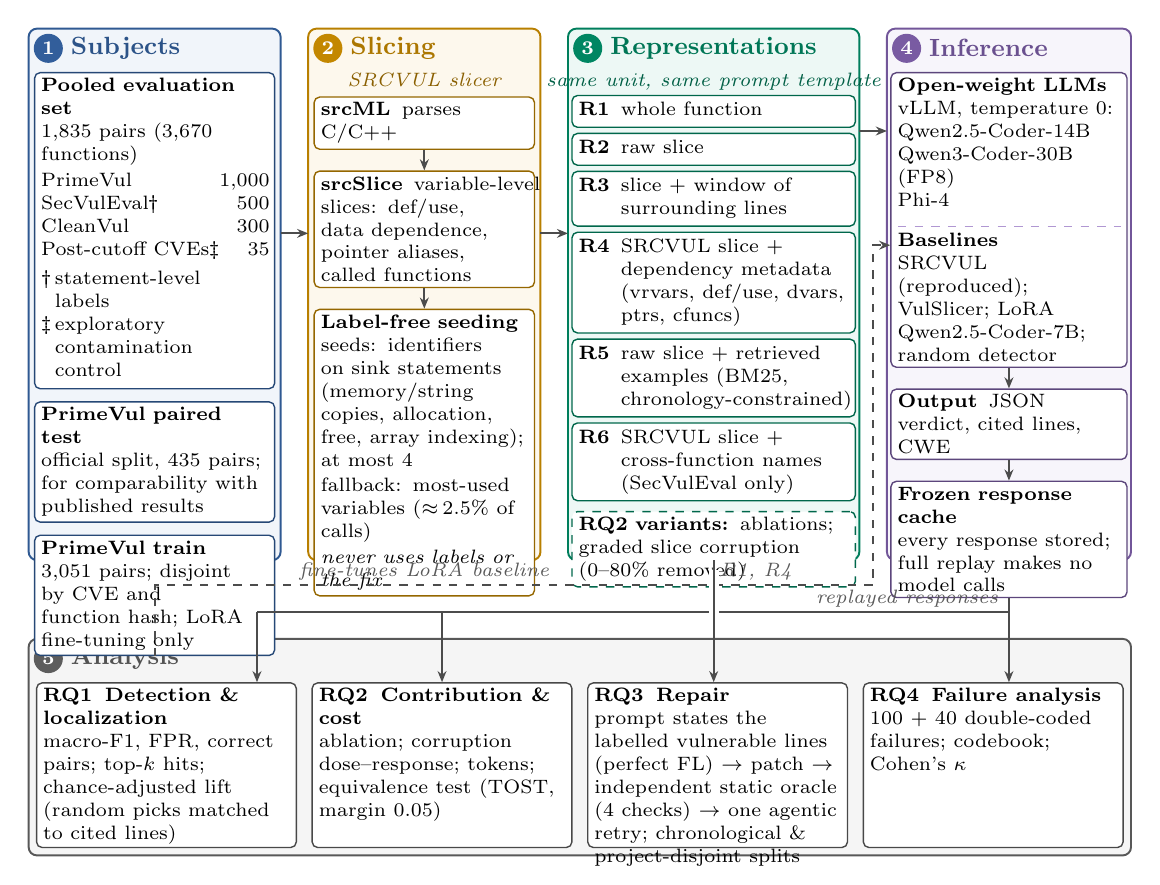
\begin{tikzpicture}[font=\bodyfont]

%================ PANEL FRAMES =================
\draw[panel=cData]  (0,0)     rectangle (3.2,-\H);
\draw[panel=cSlice] (3.55,0)  rectangle (6.5,-\H);
\draw[panel=cRep]   (6.85,0)  rectangle (10.55,-\H);
\draw[panel=cInf]   (10.9,0)  rectangle (14.0,-\H);
\draw[panel=cAna]   (0,\Ay)   rectangle (14.0,\Ab);

\paneltitle{0}{0}{1}{cData}{Subjects}
\paneltitle{3.55}{0}{2}{cSlice}{Slicing}
\paneltitle{6.85}{0}{3}{cRep}{Representations}
\paneltitle{10.9}{0}{4}{cInf}{Inference}
\paneltitle{0}{\Ay}{5}{cAna}{Analysis}

%================ 1 SUBJECTS =================
\node[box=cData,text width=2.88cm] (pool) at (1.6,-0.55) {%
  \textbf{Pooled evaluation set}\\
  1,835 pairs (3,670 functions)\\[1pt]
  \begin{tabular}{@{}l@{}r@{}}
  \makebox[2.15cm][l]{PrimeVul} & 1,000\\
  SecVulEval\textdagger & 500\\
  CleanVul & 300\\
  Post-cutoff CVEs\textdaggerdbl & 35
  \end{tabular}\\[1pt]
  \begin{tabular}{@{}l@{\,}p{2.6cm}@{}}
  \textdagger & statement-level labels\\
  \textdaggerdbl & exploratory contamination control
  \end{tabular}};
\node[box=cData,text width=2.88cm,below=0.15cm of pool] (test) {%
  \textbf{PrimeVul paired test}\\
  official split, 435 pairs; for comparability with published results};
\node[box=cData,text width=2.88cm,below=0.15cm of test] (train) {%
  \textbf{PrimeVul train}\\
  3,051 pairs; disjoint by CVE and function hash; LoRA fine-tuning only};

%================ 2 SLICING =================
\node[note=cSlice!60!black,anchor=north] at (5.025,-0.5) {\sv{} slicer};
\node[box=cSlice,text width=2.63cm] (srcml) at (5.025,-0.86) {%
  \textbf{srcML}\enspace parses C/C++};
\node[box=cSlice,text width=2.63cm,below=0.26cm of srcml] (srcslice) {%
  \textbf{srcSlice}\enspace variable-level slices: def/use, data dependence, pointer aliases, called functions};
\node[box=cSlice,text width=2.63cm,below=0.26cm of srcslice] (seed) {%
  \textbf{Label-free seeding}\\
  seeds: identifiers on sink statements (memory/string copies, allocation, free, array indexing); at most~4\\[1pt]
  fallback: most-used variables (${\approx}\,2.5\%$ of calls)\\[1pt]
  \textit{never uses labels or the fix}};
\draw[flow] (srcml) -- (srcslice);
\draw[flow] (srcslice) -- (seed);

%================ 3 REPRESENTATIONS =================
\node[note=cRep!60!black,anchor=north] at (8.7,-0.5) {same unit, same prompt template};
\node[box=cRep,text width=3.43cm,inner ysep=1.6pt] (r1) at (8.7,-0.84) {\rrow{R1}{whole function}};
\node[box=cRep,text width=3.43cm,inner ysep=1.6pt,below=0.06cm of r1] (r2) {\rrow{R2}{raw slice}};
\node[box=cRep,text width=3.43cm,inner ysep=1.6pt,below=0.06cm of r2] (r3) {\rrow{R3}{slice + window of surrounding lines}};
\node[box=cRep,text width=3.43cm,inner ysep=1.6pt,below=0.06cm of r3] (r4) {\rrow{R4}{\sv{} slice + dependency metadata (vrvars, def/use, dvars, ptrs, cfuncs)}};
\node[box=cRep,text width=3.43cm,inner ysep=1.6pt,below=0.06cm of r4] (r5) {\rrow{R5}{raw slice + retrieved examples (BM25, chronology-constrained)}};
\node[box=cRep,text width=3.43cm,inner ysep=1.6pt,below=0.06cm of r5] (r6) {\rrow{R6}{\sv{} slice + cross-function names (SecVulEval only)}};
\node[box=cRep,text width=3.43cm,below=0.12cm of r6,dashed] (var)
  {\textbf{RQ2 variants:} ablations; graded slice corruption (0--80\% removed)};

%================ 4 INFERENCE =================
\node[box=cInf,text width=2.83cm] (det) at (12.45,-0.55) {%
  \textbf{Open-weight LLMs}\\
  vLLM, temperature 0:\\
  Qwen2.5-Coder-14B\\
  Qwen3-Coder-30B (FP8)\\
  Phi-4\\[-1pt]
  \tikz\draw[cInf!70,dashed,line width=0.4pt](0,0)--(2.83cm,0);\\[-1pt]
  \textbf{Baselines}\\
  \sv{} (reproduced); VulSlicer; LoRA Qwen2.5-Coder-7B; random detector};
\node[box=cInf,text width=2.83cm,below=0.26cm of det] (out) {%
  \textbf{Output}\enspace JSON verdict, cited lines, CWE};
\node[box=cInf,text width=2.83cm,below=0.26cm of out] (cache) {%
  \textbf{Frozen response cache}\\ every response stored; full replay makes no model calls};
\draw[flow] (det) -- (out);
\draw[flow] (out) -- (cache);

%================ 5 ANALYSIS =================
\def\Ry{\Ay-0.55}
\tikzset{rq/.style={box=cAna}}
\newcommand{\rqtext}[1]{\parbox[t][1.95cm][t]{3.13cm}{\raggedright\hyphenpenalty=10000 #1}}
\node[rq] (rq1) at (1.75,\Ry) {\rqtext{%
  \textbf{RQ1\enspace Detection \& localization}\\
  macro-F1, FPR, correct pairs; top-$k$ hits; chance-adjusted lift (random picks matched to cited lines)}};
\node[rq] (rq2) at (5.25,\Ry) {\rqtext{%
  \textbf{RQ2\enspace Contribution \& cost}\\
  ablation; corruption dose--response; tokens; equivalence test (TOST, margin 0.05)}};
\node[rq] (rq3) at (8.75,\Ry) {\rqtext{%
  \textbf{RQ3\enspace Repair}\\
  prompt states the labelled vulnerable lines (perfect FL) $\rightarrow$ patch $\rightarrow$ independent static oracle (4~checks) $\rightarrow$ one agentic retry; chronological \& project-disjoint splits}};
\node[rq] (rq4) at (12.25,\Ry) {\rqtext{%
  \textbf{RQ4\enspace Failure analysis}\\
  100 + 40 double-coded failures; codebook; Cohen's $\kappa$}};

%================ INTER-PANEL ARROWS =================
\draw[flow] (3.2,-2.6) -- (3.55,-2.6);
\draw[flow] (6.5,-2.6) -- (6.85,-2.6);
\draw[flow] (10.55,-1.3) -- (10.9,-1.3);

% train split -> LoRA baseline
\def\ytr{-\H-0.32}
\def\ylo{-2.75}
\draw[flow,dashed] (train.south) -- (train.south |- 0,\ytr) -- (10.725,\ytr)
   -- (10.725,\ylo) -- (det.west |- 0,\ylo);
\node[note=black!65,anchor=south] at (5.025,\ytr) {fine-tunes LoRA baseline};

% cache -> RQ1, RQ2, RQ4 (bus)
\def\ybus{-\H-0.66}
\draw[line width=0.7pt,draw=black!70] (cache.south) -- (cache.south |- 0,\ybus) -- (2.9,\ybus);
\draw[flow] (cache.south |- 0,\ybus) -- (cache.south |- rq4.north);
\draw[flow] (5.25,\ybus) -- (5.25,0 |- rq2.north);
\draw[flow] (2.9,\ybus) -- (2.9,0 |- rq1.north);
\node[note=black!65,anchor=south east] at (12.37,\ybus) {replayed responses};

% R1, R4 -> RQ3 (drawn last; white halo makes it hop over the lines)
\draw[white,line width=3.6pt] (8.7,-\H-0.12) -- (8.7,\Ay+0.06);
\draw[flow] (8.7,-\H) -- (8.7,0 |- rq3.north);
\node[note=black!65,anchor=south west] at (8.72,\ytr) {R1, R4};

\end{tikzpicture}
\end{document}
